\section{Kommunikation}

\subsection{Client <-> Server} 
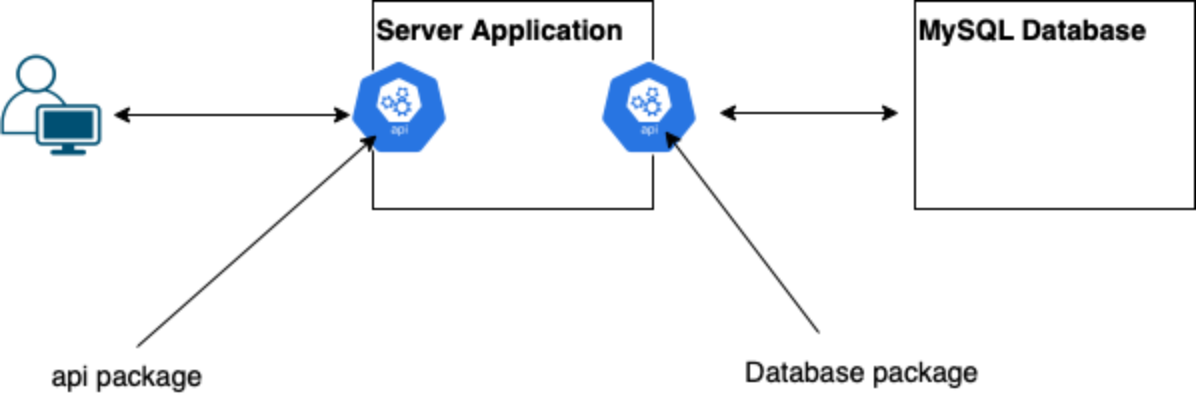
\includegraphics[width=1\textwidth]{res/Kommunikation.png}
Die Kommunikation zwischen Client und Server erfolgt über das \nameref{API}, bei der die Klasse FrontendAPI 
als RESTful API über JSON mit dem Client kommuniziert und das Database Package die Kommunikation 
zwischen der Datenbank und der Server Application regelt. Beide Schnittstellen sind zugleich Fassaden, die die Kommunikation
zwischen den einzelnen Subsystemen regeln.
Hier ist also eine horizontale Schichtenarchitektur vorhanden.

%Frontend API
\subsubsection{Frontend API}
Hinweis: Json Objekte werden in Python nativ als String interpretiert. Das ist dementsprechend im Entwurf aber durch die 
Benennung der Parameter klar, da json Objekte immer mit json\texttt{\_}details o.Ä. beschrieben werden.
Mithilfe von Flask läuft auf dem Hostserver eine RESTful API, die 

%Lukas zum Database package
\subsubsection{Database package}
\subsection{Server <-> Airflow API}

\newpage